\documentclass[a4paper,11pt,notitlepage]{report}

\usepackage{graphicx}
\usepackage[utf8]{inputenc}
\usepackage[T1]{fontenc}
\usepackage[ngerman]{babel}
\usepackage{bibgerm}
\usepackage{amsmath,amssymb,amsthm}
\usepackage{color}
\usepackage{enumerate}
\usepackage{tabularx}
\usepackage{subfig}
\usepackage{fancyhdr}
\usepackage{upgreek}
\usepackage[pdftex,pdfpagelabels,colorlinks,backref,pagebackref]{hyperref}
\usepackage{tikz} % SELBST HINZUGEFÜGT
\usepackage{graphicx}
\usepackage{framed}
\usepackage{lmodern}
% == Set the heading style ===================================================
\setlength{\headheight}{14pt}
\pagestyle{fancyplain}
\renewcommand{\chaptermark}[1]{\markboth{#1}{}}
\renewcommand{\sectionmark}[1]{\markright{\thesection\ #1}}
\lhead[\fancyplain{}{\thepage}]{\fancyplain{}{\rightmark}}
\rhead[\fancyplain{}{\leftmark}]{\fancyplain{}{\thepage}}
\cfoot{}
\renewcommand{\headrulewidth}{0.4pt}
% ============================================================================

% == Set correct values for fitting floats ===================================
\tolerance=2000
\emergencystretch=10pt

\setcounter{topnumber}{3}
\setcounter{totalnumber}{5}
\setcounter{bottomnumber}{2}

% To make those darn floats fit where they should
\setcounter{totalnumber}{9}
\setcounter{topnumber}{9}
\setcounter{bottomnumber}{9}
\renewcommand{\textfraction}{0.00}
\renewcommand{\topfraction}{1.0}
\renewcommand{\bottomfraction}{1.0}
% ============================================================================

% == German definitions for theorems etc. ==================================== 
\newtheorem{definition}{Definition}[chapter]
\newtheorem{theorem}{Satz}[chapter]
\newtheorem{lemma}{Lemma}[chapter]
\newtheorem{proposition}{Proposition}[chapter]
\newtheorem{corollary}{Korollar}[chapter]
\newtheorem{observation}{Beobachtung}[chapter]
\newtheorem{fact}{Fakt}[chapter]
\newtheorem{remark}{Bemerkung}[chapter]
\newtheorem{example}{Beispiel}[chapter]
% ============================================================================

% == Abkürzungen für die reellen, natürlichen, ganzen,... Zahlen =============
\newcommand{\R}{{\ensuremath{\mathbb{R}}}}
\newcommand{\N}{{\ensuremath{\mathbb{N}}}}
\newcommand{\Z}{{\ensuremath{\mathbb{Z}}}}
\newcommand{\C}{{\ensuremath{\mathbb{C}}}}
\newcommand{\Q}{{\ensuremath{\mathbb{Q}}}}
\newcommand{\F}{{\ensuremath{\mathbb{F}}}}
\newcommand{\Prim}{{\ensuremath{\mathbb{P}}}}
% ============================================================================

% == Makros für Autorenname und -adresse =====================================
\newcommand{\myaddress}[6]{%
  \parbox{\textwidth}{\textbf{\large #1}\\
    #2\\ #3\\ #4\\ 
    \ifthenelse{\equal{#5}{}}{}{Email: \href{mailto:#5}{\texttt{#5}}\\}
    \ifthenelse{\equal{#6}{}}{}{WWW: \href{#6}{\path|#6|}\\}
  } 
}

\newcommand{\myauthor}[1]{%
  \addtocontents{toc}{\protect\hspace{3.35ex}%
  \textsl{#1}\par}\vspace{-4ex}\quad\hfill\textsl{\Large #1}\vspace{8ex}}

\newcommand{\myname}[1]{\Large #1}

%%%%%%%%%%%%%%%%%%%%%%%%%%%%%%%%%%%%%%%%%%%%%%%%%%
% Tragen Sie in der folg. Zeile Ihren Namen ein: %
%%%%%%%%%%%%%%%%%%%%%%%%%%%%%%%%%%%%%%%%%%%%%%%%%%

\newcommand{\OO}{{\ensuremath{\mathcal{O}}}}

\renewcommand{\thechapter}{\Roman{chapter}}
\renewcommand{\thesection}{\arabic{section}}


%\newenvironment{Kasten}[1]
%{
%\hspace{0.05\linewidth}
%\begin{center}
%\begin{minipage}{0.95\linewidth}
%\setlength{\fboxsep}{10pt}
%\definecolor{shadecolor}{rgb}{0.9,1,1}
%\definecolor{framecolor}{gray}{0}
%\def\FrameCommand{\fcolorbox{framecolor}{shadecolor}}
%\MakeFramed {\FrameRestore}
%\subsection*{#1}
%}
%{
%\endMakeFramed
%\end{minipage}
%\end{center}
%}

\newtheorem{Kasten}{Definition}[chapter]


\newenvironment{bsp}[1]
{
\setlength{\fboxsep}{10pt}
\subsection*{Beispiel: #1}
\begin{upshape}
}
{
\end{upshape}
}

\begin{document}
\shorthandoff{"}
\setcounter{chapter}{0}

\begin{titlepage}
	\begin{center}	
		\LARGE \textbf{{Einführung in die Geometrie und Topologie - Definitionen und Sätze -} \\[5ex] 
    		{\Large Vorlesung im Wintersemester 2011/2012\\[5ex]}}
	\end{center}
	\begin{center}
		\Large Sarah Lutteropp, Simon Bischof
	\end{center}
	\begin{center}
		\today
	\end{center}
	\vspace{2cm}
	\begin{center}
		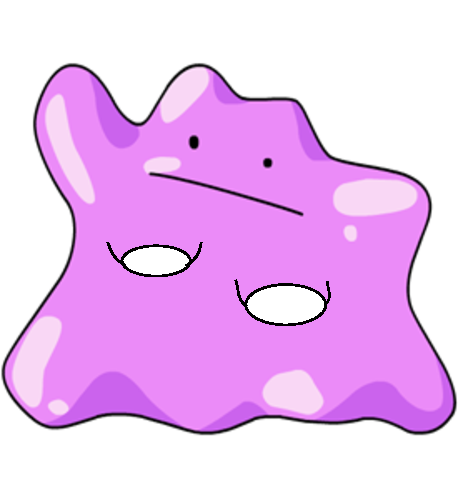
\includegraphics[width=0.8\textwidth]{images/ditto_loecher.pdf}
	\end{center}
\end{titlepage}
%\maketitle
\setcounter{tocdepth}{1}
\tableofcontents

\section*{Zusammenfassung}
Dies ist ein Mitschrieb der Vorlesung “Einführung in die Geometrie und Topologie” vom Wintersemester 2011/2012 am Karlsruher Institut für Technologie, die von Herrn Prof. Dr. Wilderich Tuschmann gehalten wird.

\chapter{Definitionen und Sätze aus der Vorlesung}

\begin{Kasten}[Topologischer Raum]
Ein \underline{topologischer Raum} $X$ ist gegeben durch eine Menge $X$ und ein System $\OO$ von Teilmengen von $X$, den so genannten \underline{offenen Mengen} von $X$, welches unter beliebigen Vereinigungen und endlichen Durchschnitten abgeschlossen ist und $X$ und die leere Menge $\emptyset$ als Elemente enthält.
\newline
$X$ Menge, $\OO \subset \mathcal{P}(X) \colon$
\begin{enumerate}[(1)]
	\item $O_1, O_2 \in \OO \Rightarrow O_1 \cap O_2 \in \OO$
	\item $O_\alpha \in \OO, \alpha \in A, A \text{ Indexmenge} \Rightarrow \bigcup\limits_{\alpha \in A}{O_\alpha} \in \OO$
	\item $X, \emptyset \in \OO$
\end{enumerate}
\end{Kasten}

\begin{Kasten}[Metrischer Raum]
Ein \underline{metrischer Raum} $X$ ist eine Menge $X$ mit einer Abbildung $d \colon X \times X \rightarrow \R$, der \underline{"Metrik"} auf $X$, die folgende Eigenschaften erfüllt:
$\forall x,y,z \in X$ gilt:
\begin{enumerate}[(1)]
	\item $d(x,y) = d(y,x)$ \underline{"Symmetrie"}
	\item $d(x,y) = 0 \Leftrightarrow x = y, d(x,y) \geq 0$ \underline{"Definitheit"}
	\item $d(x,z) \leq d(x,y) + d(y,z)$ \underline{"Dreiecksungleichung"}
\end{enumerate}
\end{Kasten}

\begin{Kasten}[Stetigkeit]
Eine Abbildung $F \colon X \rightarrow Y$ zwischen topologischen Räumen $X$ und $Y$ heißt \underline{stetig}, falls die F-Urbilder offener Mengen in $Y$ offene Teilmengen von $X$ sind.
%\end{Kasten}
\end{Kasten}

\begin{Kasten}[Homotopie]
Eine \underline{Homotopie} $H \colon f \simeq g$ zwischen zwei (stetigen) Abbildungen $f,g \colon X \rightarrow Y$ ist eine (stetige) Abbildung $$H \colon X \times I \rightarrow Y, (x,t) \mapsto H(x,t)$$ 
mit $H(x,0) = f(x) \text{ und } H(x,1) = g(x) \quad \forall x \in X$.
\newline
(Hier ist $I = [0,1] \subset \R$)
\newline
$f$ und $g$ heißen dann \underline{homotop}, in Zeichen: $f \simeq g$.
\end{Kasten}

\begin{Kasten}[Homotope Abbildungen $f,g \colon X \rightarrow Y$]
	Zwei (stetige) Abbildungen heißen \underline{homotop}, in Zeichen: $f \simeq g$, falls eine Homotopie mit Anfang $f$ und Ende $g$ existiert.
\end{Kasten}

\begin{Kasten}[Nullhomotopie]
Eine stetige Abbildung $f \colon X \rightarrow Y$ heißt \underline{nullhomotop}, falls sie homotop zu einer konstanten Abbildung ist.
\end{Kasten}

\begin{corollary}
Jede stetige Abbildung $f \colon X \rightarrow \R^n$ ist nullhomotop, d.h. für jeden topologischen Raum $X$ besteht $[X, \R^n]$, $n$ beliebig, nur aus einem Punkt!
\end{corollary}

\begin{Kasten}[Teilraumtopologie]
Es sei $(X, \OO)$ topologischer Raum und $A \subset X$. Die auf $A$ durch
$$\OO \Big |_{A} := \{U \cap A \mid U \in \OO \}$$
induzierte Topologie heißt \underline{Teilraumtopologie} und der dadurch gegebene topologische Raum $(A, \OO \Big |_{A})$ heißt \underline{Teilraum} von $(X, \OO)$.
\end{Kasten}

\begin{Kasten}[Abgeschlossenheit]
	$A \subset X, X$ topologischer Raum, heißt \underline{abgeschlossen} $$:\Leftrightarrow X \backslash A \text{ ist offen.}$$
\end{Kasten}

\begin{Kasten}[Umgebung]
	Ist $X$ topologischer Raum und $x \in X$, so heißt jede \underline{offene} Teilmenge $O \subset X$ mit $x \in O$ eine \underline{Umgebung} von $x$.
%\end{Kasten}
\end{Kasten}

\begin{Kasten}[Basis]
	Ist $(X, \OO)$ topologischer Raum mit $\mathcal{B} \subset \OO$, 
	\newline
	so heißt $\mathcal{B}$ \underline{Basis der Topologie} $:\Leftrightarrow$ Jede (nichtleere) offene Menge ist Vereinigung von Mengen aus $\mathcal{B}$.
\end{Kasten}

\begin{Kasten}[Produkt-Topologie]
	Sind $(X, \OO_X)$ und $(Y, \OO_Y)$ topologische Räume, so bildet $$\mathcal{B}_{X \times Y} := \{U \times V \mid U \in \OO_X, V \in \OO_Y\}$$
	die Basis einer Topologie für die Menge $X \times Y$, und diese heißt \underline{Produkt-Topologie auf $X \times Y$}.
	\newline
	Versehen mit der Produkt-Topologie ist $X \times Y$ sebst ein topologischer Raum und für gegebene $X, Y$ denkt man sich $X \times Y$ stillschweigend mit der Produkt-Topologie versehen.
\end{Kasten}

\begin{Kasten}[Feiner und gröber]
	Sind $\OO_1$ und $\OO_2$ Topologien auf $X$ und $\OO_1 \subset \OO_2$, 
	\newline so heißt $\OO_2$ \underline{feiner} als $\OO_1$ und $\OO_1$ \underline{gröber} als $\OO_2$.
\end{Kasten}

\begin{Kasten}[$\epsilon$-Ball, Sphäre]
	Für einen metrischen Raum $(X,d)$ und $\epsilon > 0$ sei für $p \in X$
	\begin{itemize}
		\item $B_\epsilon(p):=\{x \in C \mid d(p,x) < \epsilon \}$ der \underline{offene $\epsilon$-Ball um $p$}
		\item $D_\epsilon(p):=\{x \in C \mid d(p,x) \leq \epsilon \}$ der \underline{abgeschlossene $\epsilon$-Ball um $p$}
		\item $S_\epsilon(p):=\{x \in C \mid d(p,x) = \epsilon \}$ die \underline{ $\epsilon$-Sphäre} um $p$ (oder \underline{Sphäre vom Radius $\epsilon$} um $p$)
	\end{itemize}
\end{Kasten}

\begin{Kasten}[Metrischer Unterraum]
	Ist $(X,d)$ metrischer Raum und $A \subset X$, so heißt der metrische Raum $(A, d \big |_{A \times A})$ \underline{(metrischer) Unterraum von $X$}.
\end{Kasten}

\begin{Kasten}[Beschränktheit, Durchmesser]
	$A \subset (X,d)$ heißt \underline{beschränkt} \newline $:\Leftrightarrow \exists 0 < \rho \in \R \colon d(x,y) < \rho  \text{   } \forall x,y \in A$
	\newline
	Das Infimum, diam $A$, dieser $\rho$ heißt dann \underline{Durchmesser von $A$}.
	\newline
	\begin{center}
	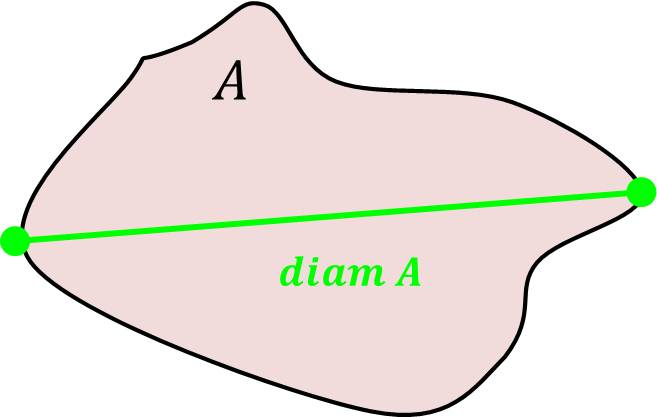
\includegraphics[width=0.4\textwidth]{images/Durchmesser.jpg}
	\end{center}
\end{Kasten}

\begin{Kasten}[Abstand]
	$(X,d)$ sei metrischer Raum und $A \subset X, p \in X$.
	$$d(p,A) := dist(p,A):= \inf \{d(p,a) \mid a\in A \}$$
	heißt \underline{Abstand von $p$ und $A$}.
\end{Kasten}

\begin{Kasten}[Innerer Punkt, äußerer Punkt, Randpunkt]
	Für $p \in A \subset X$, $X$ topologischer Raum, heißt $p$
	\newline
	\begin{enumerate}[(1)]
		\item \underline{innerer Punkt} von $A$, falls es eine in $A$ enthaltene Umgebung $U$ um $p$ gibt. 
		\item \underline{äußerer Punkt}, falls eine zu $p$ disjunkte Umgebung $V$ in $X$ existiert.
		\item \underline{Randpunkt von $A$}, falls jede Umgebung von $p$ nichtleeren Durchschnitt mit $A$ und $X \backslash A$ hat.
	\end{enumerate}
\end{Kasten}
	
\begin{Kasten}[Inneres]
	Für $A \subset X$ heißt die größte in $X$ offene und in $A$ enthaltene Teilmenge $\mathring A$ \underline{Inneres von $A$}.
\end{Kasten}

\begin{Kasten}[Abschluss]
	Der \underline{Abschluss} $\bar{A}$ von $A$ ist $X \backslash \left ( \mathring {(X \backslash A} ) \right )$.
\end{Kasten}

\begin{Kasten}[Rand]
	Der \underline{Rand} $\partial A$ von $A$ ist $$\partial A := \bar{A} \backslash \mathring A,$$ d.h. Rand $A$ = \{ Randpunkte von A \}.
\end{Kasten}

\begin{Kasten}[Stetigkeit]
	$f \colon X \rightarrow Y$ ist stetig $:\Leftrightarrow \forall$ offenen Mengen in $Y$ ist das Urbild unter $f$ offene Menge in $X$.
\end{Kasten}

\begin{Kasten}[Stetigkeit]
	$f \colon X \rightarrow Y$ ist stetig in $x \in X$
	$$:\Leftrightarrow \forall \text{ Umgebungen } V \text{ von } f(x) \quad \exists \text{ Umgebung } U \text{ von } x \text{ mit }$$ $$f(U) \subset V.$$
	\newline
\end{Kasten}

\begin{Kasten}[Isometrische Einbettung, Isometrie]
	Sind $X,Y$ metrische Räume, so heißt eine Abbildung $f \colon X \rightarrow Y$ \underline{isometrische Einbettung}
	\newline	
	 $: \Leftrightarrow \forall x, x^\prime \in X$ gilt $d_Y \left ( f(x), f(x^\prime) \right ) = d_X (x, x^\prime)$.
	\newline
	Eine isometrische Einbettung ist immer injektiv.
	\newline
	Ist $f$ zusätzlich \underline{bijektiv}, so heißt $f$ \underline{\underline{Isometrie}}. 
\end{Kasten}

\begin{Kasten}[Homöomorphismus]
	Eine invertierbare Abbildung $f \colon X \rightarrow Y$ topologischer Räume heißt \underline{Homöomorphismus}, falls $f$ und $f^{-1}$ stetig sind.
\end{Kasten}


\begin{Kasten}[homöomorph]
	Zwei topologische Räume $X$ und $Y$ heißen \underline{homöomorph} oder \underline{vom gleichen Homöomorphietyp}, in Zeichen $X \cong Y$, falls es einen Homöomorphismus $f \colon X \rightarrow Y$ gibt.
\end{Kasten}

\begin{Kasten}{Einbettung}
	$f \colon X \rightarrow Y$ stetig heißt \underline{Einbettung} $$:\Leftrightarrow X \overset{f}{\rightarrow}f(X) \subset Y \text{ Homöomorphismus.}$$
\end{Kasten}

\begin{Kasten}{Äquivalenz von Einbettungen}
	Zwei Einbettungen $f,g \colon X \rightarrow Y$ heißen \underline{äquivalent} $:\Leftrightarrow \exists \text{ Homöomorphismen } h_X \colon X \rightarrow X, h_Y \colon Y \rightarrow Y \text{ mit } g \circ h_X = h_Y \circ f$, d.h. dass das Diagramm 
		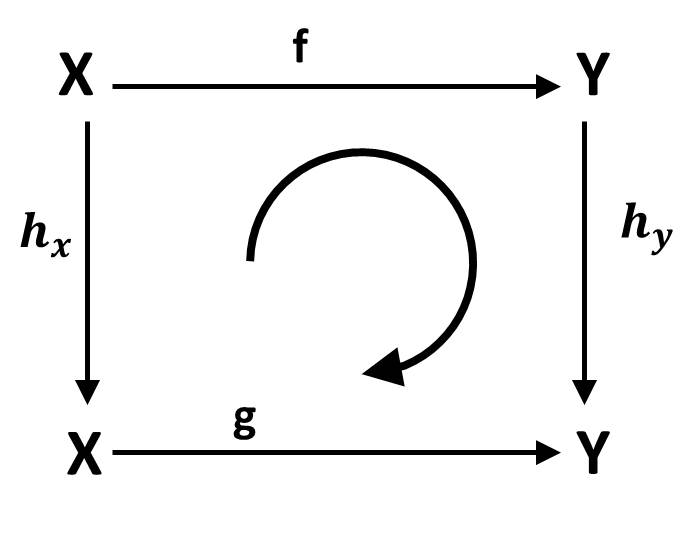
\includegraphics[scale=0.3]{images/homotopieaequivalenz.jpg} kommutiert.
\end{Kasten}

\begin{Kasten}{Knoten}
	Eine Einbettung $S^1 \rightarrow \R^3$ heißt \underline{Knoten}.
\end{Kasten}

\begin{Kasten}{zusammenhängend}
	Ein topologischer Raum heißt \underline{zusammenhängend} $:\Leftrightarrow$ Die einzigen in $X$ gleichzeitig offenen und abgeschlossenen Teilmengen sind $\emptyset$ und $X$.
	\newline
	Ansonsten heißt $X$ \underline{un-} oder \underline{nicht zusammenhängend}.
\end{Kasten}

\begin{Kasten}{Überdeckung}
	Eine Familie $\mathcal{U} = \{U_\alpha \mid \alpha \in A\}$\footnote{$A$ Indexmenge} von Teilmengen von $X$ heißt \underline{Überdeckung von $X$} $:\Leftrightarrow X = \bigcup\limits_{\alpha \in A}{U_\alpha}$.
	\newline
	$\mathcal{U}$ heißt \underline{offene} beziehungsweise \underline{abgeschlossene} Überdeckung $\Leftrightarrow$ alle $U_\alpha$ sind offen beziehungsweise abgeschlossen.
	\newline
	Für $X^\prime \subset X$ heißt eine Familie $\mathcal{U} = \{U_\alpha\}$ wie oben Überdeckung von $X^\prime$ $:\Leftrightarrow X^\prime \subset \bigcup\limits_{\alpha \in A}{U_\alpha}$.
	\newline
\end{Kasten}

\begin{Kasten}{Partition}
	Eine \underline{Partition} oder \underline{Zerlegung} einer Menge ist eine Überdeckung dieser Menge durch paarweise disjunkte, nichtleere Teilmengen.
	\newline
\end{Kasten}

\begin{Kasten}{Zusammenhangskomponente}
	Eine \underline{Zusammenhangskomponente} eines topologischen Raumes $X$ ist eine im Sinne der Inklusion von Mengen maximale zusammenhängende Teilmenge von $X$.
\end{Kasten}

\begin{theorem}
	Stetige Bilder zusammenhängender Mengen sind zusammenhängend.
	\newline
	(D.h.: Ist $f \colon X \rightarrow Y$ stetig und $X$ zusammenhängend, so auch $f(X)\subset Y$.)
\end{theorem}

\begin{corollary}
	Zusammenhang bleibt unter Homöomorphismen erhalten, und ebenso die Zahl der Zusammenhangskomponenten.
\end{corollary}

\begin{corollary}{Zwischenwertsatz:}
	Eine stetige Funktion $f \colon [a,b] \rightarrow \R$ nimmt jeden Wert zwischen $f(a)$ und $f(b)$ an.
\end{corollary}

\begin{Kasten}{Weg, Anfangspunkt, Endpunkt}
	ein \underline{Weg} in einem topologischen Raum $X$ ist eine stetige Abbildung $\gamma \colon [0,1] \rightarrow X$, und $\gamma(0)$ heißt \underline{Anfangs-}, $\gamma(1)$ \underline{Endpunkt}.
	\newline
\end{Kasten}

\begin{Kasten}{Wegzusammenhang}
	$X$ heißt \underline{wegzusammenhängend} $$:\Leftrightarrow \text{ Zu je zwei Punkten } x,x^\prime \in X \quad \exists \text{ Weg } \gamma \colon [0,1] \rightarrow X$$ $$\text{ mit } \gamma(0)=x, \gamma(1)=x^\prime.$$
\end{Kasten}

\begin{Kasten}{Kompaktheit}
	Ein topologischer Raum $X$ heißt \underline{kompakt}, falls jede offene Überdeckung von $X$ eine endliche Teilüberdeckung enthält.
\end{Kasten}

\begin{Kasten}{$T_1$-Raum}
Ein topologischer Raum $X$ heißt \underline{$T_1$-Raum} bzw. \underline{erfüllt das erste Trennungsaxiom} $:\Leftrightarrow$ Für je zwei verschiedene Punkte von $X$ existiert für jeden dieser Punkte eine Umgebung in $X$, die den anderen nicht enthält.
\newline
$\forall x \neq y \in X \exists U = U_X \colon y \notin U_X$ 
\end{Kasten}

\begin{Kasten}{$T_2$-Raum}
	$X$ heißt \underline{Hausdorff}- oder \underline{$T_2$-Raum} bzw. \underline{erfüllt das zweite Trennungsaxiom} $:\Leftrightarrow$ Je zwei verschiedene Punkte in $X$ besitzen disjunkte Umgebungen.
	\newline
	$\forall x \neq y \in X \exists U_x \ni x, U_y \ni y$ mit $U_x \cap U_y = \emptyset$
\end{Kasten}

\begin{Kasten}{Grenzwert}
Ist $(x_n)_{n \in \N}$ eine Folge von Punkten in einem topologischen Raum $X$, so heißt $x \in X$ \underline{Grenzwert} der Folge $(x_n)$ genau dann, wenn zu jeder Umgebung $U$ von $x$ ein $N \in \N$ existiert mit $x_n \in U \quad \forall n \geq N$. 
\newline
\end{Kasten}
\begin{Kasten}{Umgebungsbasis}
	Ist $X$ topologischer Raum und $x \in X$, so ist eine \underline{Umgebungsbasis} oder \underline{Basis von $X$} \underline{\underline{in $x$}} eine Familie von Umgebungen von $x$, sodass \underline{jede} Umgebung von $x$ eine Umgebung aus der Familie enthält.
\end{Kasten}

\begin{Kasten}{Abzählbarkeitsaxiome, Separabilität}
	$X$ \underline{erfüllt das erste Abzählbarkeitsaxiom}
	$:\Leftrightarrow$ jeder Punkt $x \in X$ besitzt eine abzählbare Basis.
	\newline
	$X$ \underline{erfüllt das zweite Abzählbarkeitsaxiom}
	$:\Leftrightarrow$ $X$ selbst besitzt eine abzählbare Basis.
	\newline
	$X$ heißt \underline{separabel} $:\Leftrightarrow$ $X$ enthält eine abzählbare und dichte ($\bar{A} = X$) Menge $A$.
\end{Kasten}
 
\begin{Kasten}{Lokale Kompaktheit}
$X$ heißt \underline{\underline{lokal} kompakt} \newline $:\Leftrightarrow$ Jeder Punkt $x \in X$ besitzt eine Umgebung $U$, sodass $\overline{U}$ kompakt ist.
\end{Kasten} 

\begin{Kasten}{Lokale Endlichkeit}
	Eine Familie $\Gamma$ von Teilmengen eines topologischen Raumes $X$ heißt \underline{lokal endlich} $:\Leftrightarrow \forall x \in X \quad \exists U = U(x) \colon A \cap U = \emptyset \quad \forall A \in \Gamma$ bis auf endlich viele $A$.
\end{Kasten}
 
\begin{Kasten}{Verfeinerung}
	$\Gamma, \Delta$ Überdeckungen von $X$. $\Delta$ heißt \underline{Verfeinerung} von $\Gamma$ \newline $:\Leftrightarrow \forall A \in \Delta \exists B \in \Gamma \colon A \subset B$.
\end{Kasten} 

\begin{Kasten}{Parakompaktheit}
	$X$ heißt \underline{parakompakt} $:\Leftrightarrow$ Jede offene Überdeckung besitzt eine lokal endliche offene Verfeinerung. 
\end{Kasten}

\begin{Kasten}{Mannigfaltigkeit, Karte}
	Ein topologischer Raum $M$ heißt \underline{$n$-dimensionale} \underline{(topologische) Mannigfaltigkeit}, wenn gilt:
	\begin{enumerate}
		\item $M$ ist ein Hausdorff-Raum mit abzählbarer Basis der Topologie
		\item $M$ ist lokal homöomorph zu $\R^n$, d.h. zu jedem $p \in M$ existieren eine Umgebung $U=U(p) \subset_{offen} M$ und ein Homöomorphismus $\varphi \colon U \rightarrow V, V \subset_{offen} \R^n$.
			\newline
			Jedes solche Paar $(U,\varphi)$ heißt eine \underline{Karte} oder ein \underline{lokales Koordinatensystem} um $p$.
	\end{enumerate}
\end{Kasten}

\begin{Kasten}{Atlas}
	Ein \underline{Atlas} für eine topologische $n$-Mannigfaltigkeit $M$ ist eine Menge $\mathcal{A} = \{(\varphi_\alpha, U_\alpha) \mid \alpha \in \Lambda\}$\footnote{$\Lambda$ Indexmenge}
	von Karten $\varphi_\alpha \colon U_\alpha \rightarrow V_\alpha = \varphi(U_\alpha) \subset \R^n$, so dass $M = \bigcup\limits_{a \in \Lambda}{U_\alpha}$
\end{Kasten}

\begin{Kasten}{$C^k$-Atlas, Kartenwechsel}
	Ein Atlas heißt \underline{differenzierbar} \underline{von der Klasse $C^k$} (oder: $C^k$-Atlas von $M$), wenn für alle $\alpha, \beta \in \Lambda$ mit $U_\alpha \cap U_\beta \neq \emptyset$ der \underline{Kartenwechsel} $\varphi_\beta \circ \varphi_\alpha^{-1} \colon \varphi_\alpha(U_\alpha \cap U_\beta) \rightarrow \varphi_\beta(U_\alpha \cap U_\beta)$ eine $C^k$-Abbildung, also $k$-mal stetig differenzierbar ist. $(k=0,1,2,\ldots,\infty,\omega)$
	\newline
\end{Kasten}
 
\begin{Kasten}{Verträglichkeit, differenzierbare Struktur}
	Ist $M$ topologische Mannigfaltigkeit und $\mathcal{A}=\{(\varphi_\alpha,U_\alpha) \mid \alpha \in \Lambda\}$ ein $C^k$-Atlas von $M$, so heißt eine Karte $(\varphi,U)$ von $M$ \underline{mit $\mathcal{A}$ verträglich}, falls $\mathcal{A}^\prime := \mathcal{A} \cup \{(\varphi,U)\}$ ebenfalls $C^k$-Atlas ist. 
	Ein $C^k$-Atlas heißt \underline{maximal} (oder \underline{differenzierbare Struktur} (der Klasse $C^k$)), falls $\mathcal{A}$ alle mit $\mathcal{A}$ verträglichen Karten enthält.
\end{Kasten} 

\begin{Kasten}{$C^k$-Mannigfaltigkeit, glatt}
	Eine \underline{differenzierbare Mannigfaltigkeit der Klasse $C^k$} (kurz: $C^k$-Mannigfaltigkeit) ist ein Paar $(M,\mathcal{A})$ bestehend aus einer topologischen Mannigfaltigkeit $M$ und einer $C^k$-Struktur auf $M$. Eine $C^\infty$-Mannigfaltigkeit heißt auch \underline{\underline{glatt}}.
	\newline
\end{Kasten}

\begin{Kasten}{$C^l$-Abbildung}
Es seien $(M, \mathcal{A})$ eine $n$-dimensionale $C^k$-Mannigfaltigkeit, $(M^\prime, \mathcal{A}^\prime)$ eine $n^\prime$-dimensionale $C^{k^\prime}$-Mannigfaltigkeit und $l \leq \min(k,k^\prime)$. Eine stetige Abbildung $f \colon M \rightarrow M^\prime$ heißt \underline{differenzierbar} (\underline{von der Klasse $C^l$}) oder kurz: $C^l$-Abbildung, falls gilt:
$$\forall (\varphi,U) \in \mathcal{A} \text{ und } (\varphi^\prime, U^\prime) \in \mathcal{A}^\prime \text{ mit } f(U) \cap U^\prime \neq \emptyset \text{ ist}$$
$$\boxed{\varphi^\prime \circ f \circ \varphi^{-1} \colon \varphi(U \cap f^{-1}(U^\prime)) \rightarrow \varphi^\prime(f(U)\cap U^\prime)}$$
eine $C^l$-Abbildung im üblichen Sinn.
\end{Kasten}

\begin{theorem}[Äquivalente Beschreibungen einer Untermannigfaltigkeit von $\R^{n+l}$]
	Für Teilmengen $M \subset \R^{n+l}$ sind äquivalent:
	\begin{enumerate}[(a)]
		\item $\forall x_0 \in M \exists \text{ Umgebung } U = U(x_0) \subset_{offen} \R^{n+l}$ und $$f \in C^\infty(U, \R^l) := \{g \colon U \rightarrow \R^l \mid g \text{ ist } C^\infty\}\text{ mit Rang }Df(x) = l \quad \forall x \in U$$ \footnote{$Df$ ist die Jacobi-Matrix von $f$} dergestalt, dass $U \cap M = f^{-1}(0) = \{x \in U \mid f(x) = 0\}$ 
	\begin{center}
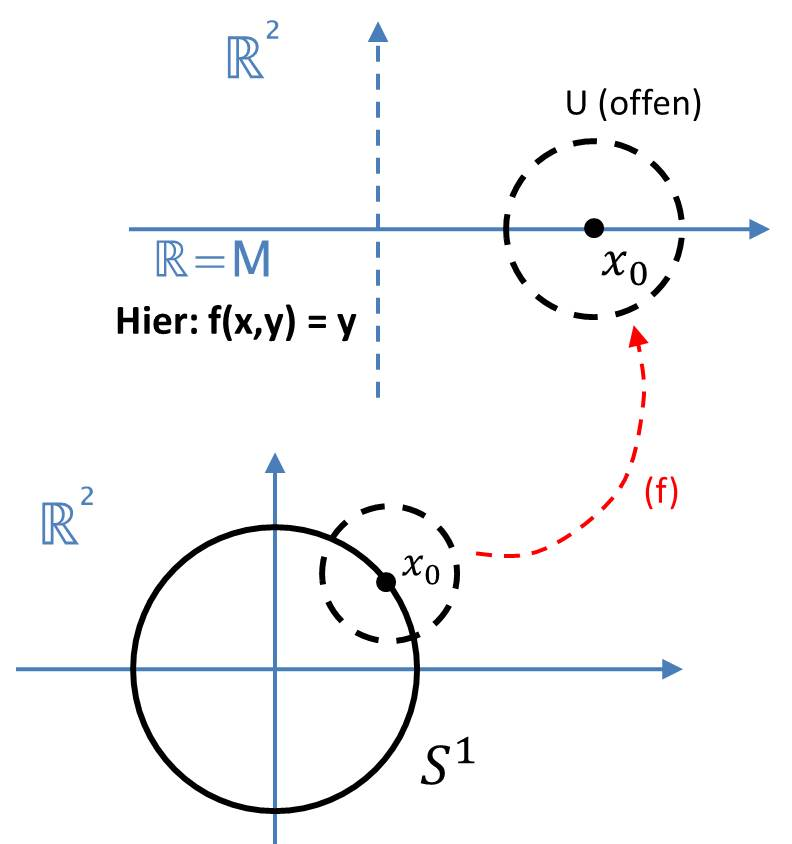
\includegraphics[scale=0.5]{images/Satz_UnterMf.jpg}
	\end{center}
		\item $\forall x_0 \in M \exists U = U(x) \subset_{offen} \R^{n+l}$ und $\varphi \colon U \rightarrow \R^{n+l}$ mit folgenden Eigenschaften:
		$\varphi(U) \subset \R^{n+l}$ ist offen, \newline $\varphi$ ist $C^\infty$-Diffeomorphismus $U \rightarrow \varphi(U)$ und $$\varphi(U \cap M) = \varphi(U) \cap (\R^n \times \{0\}) = \{(y_1, \ldots, y_{n+l}) \in \varphi(U) \mid y_{n+1} = \ldots = y_{n+l} = 0 \}$$
		\item $\forall x_0 \in M \exists U = U(x_0) \subset_{offen} \R^{n+l}, W \subset \R^n$ offen und $\psi \in C^\infty(W,U)$ mit 
			\begin{itemize}
				\item $\psi$ ist Homöomorphismus $W \rightarrow U \cap M$
				\item $D\psi(w)$ ist injektiv für alle $w \in W$
			\end{itemize}
			(Jedes solche $\psi$ heißt \underline{lokale Parametrisierung von $M$}).
	\end{enumerate}
\end{theorem}

\begin{Kasten}{Untermannigfaltigkeit}
Eine Menge $M \subset \R^{n+l}$, die eine der Bedingungen (a), (b) oder (c) erfüllt, heißt dann \underline{$n$-dimensionale} \underline{(glatte/differenzierbare) Untermannigfaltigkeit von $\R^{n+l}$}.
\end{Kasten}

\begin{theorem}{Äquivalente Beschreibung einer glatten Untermannigfaltigkeit von $\R^{n+l}$}
	Es sei $M \subseteq \R^{n+l}$. Es sind äquivalent:
	\begin{enumerate}[(a)]
		\item $\forall x_0 \in M \exists U = U(x_0) \subseteq_{\text{offen}} \R^{n+l} \text{ und } f \in C^\infty(U,\R^l)$ $\text{ mit Rang }Df(x) = l \text{ für alle } x \in U$ dergestalt, dass $U \cap M = f^{-1}(0)$.
		\item $\forall x_0 \in M \exists U = U(x) \subseteq_{\text{offen}} \R^{n+l} \text{ und } \varphi \colon U \rightarrow \R^{n+l}$ mit folgenden Eigenschaften:
			\begin{itemize}
				\item $\varphi(U) \subseteq \R^{n+l}$ ist offen
				\item $\varphi$ ist $C^\infty$-Diffeomorphismus $U \rightarrow \varphi(U)$
				\item $\varphi(U \cap M) = \varphi(U) \cap (\R^n \times \{0\})$ $= \{(y_1, \ldots, y_n) \in \varphi(U) \mid y_{n+1} = \ldots = y_{n+l} = 0\}$
			\end{itemize}
		\item $\forall x_0 \in M \exists U = U(x_0) \subseteq_{\text{offen}} \R^{n+l}$, $W \subseteq \R^n$ offen und $\psi \in C^\infty(W,U)$ mit folgenden Eigenschaften:
			\begin{itemize}
				\item $\psi$ ist Homöomorphismus $W \rightarrow U \cap M$
				\item $D\psi(w)$ ist injektiv für alle $w \in W$.
			\end{itemize}
	\end{enumerate}
\end{theorem}


\begin{theorem}{($C^\infty$-Untermannigfaltigkeiten von $\R^{n+l}$ sind $C^\infty$-Mannigfaltigkeiten)}
	Es sei $M \subseteq \R^{n+l}$ $n$-dimensionale $C^\infty$-Untermannigfaltigkeit von $\R^{n+l}$ und $\{\psi_\alpha \colon W_\alpha \rightarrow U_\alpha \cap M \mid \alpha \in \Lambda\}$ eine Menge lokaler Parametrisierungen (wie in (c)) mit $M \subseteq \bigcup\limits_{\alpha \in \Lambda}{U_\alpha}$.
	Dann ist $\mathcal{A} = \{(\psi_\alpha^{-1}, U_\alpha \cap M) \mid \alpha \in \Lambda\}$ ein $C^\infty$-Atlas und $M$ eine $C^\infty$-Mannigfaltigkeit.
\end{theorem}

\begin{Kasten}{Quotienten(raum)topologie}
	Eine Teilmenge $U \subset X/S$ heißt \underline{offen}
	$:\Leftrightarrow \pi^{-1}(U)$ ist offen in $X$
\end{Kasten}

\begin{Kasten}{Quotientenabbildung}
Ist $S$ eine Partition von $X$ in nichtleere disjunkte Teilmengen und $f \colon X \rightarrow Y$ eine Abbildung, die auf jedem Element von $S$ konstant ist, so existiert eine Abbildung $X/S \rightarrow Y$, die jedes Element $A$ von $S$ auf $f(a), a \in A,$ abbildet. \newline
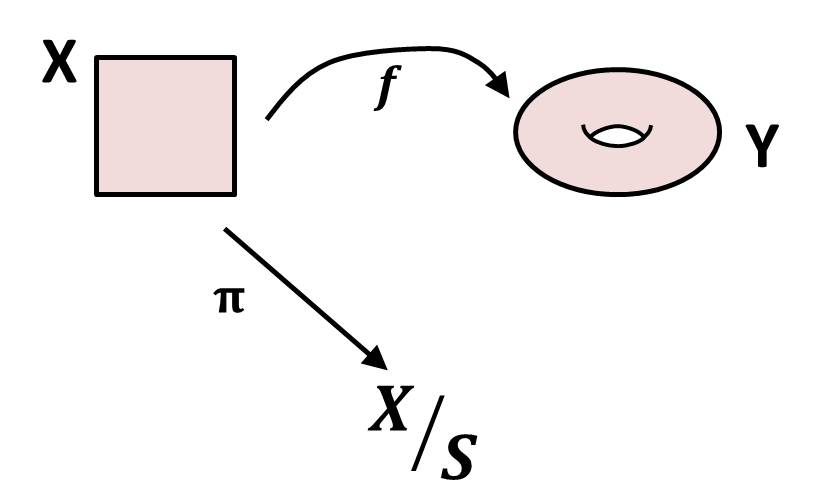
\includegraphics[scale=0.4]{images/Quotientenabbildung.jpg} \newline
Diese heißt dann \textbf{Quotientenabbildung} von $f$ nach $S$, in Zeichen $f/S$.
\end{Kasten}

\begin{corollary}
	$X$ kompakt, $Y$ Hausdorffsch und $f \colon X \rightarrow Y$ sei stetig 
	$\Rightarrow$ Der \underline{injektive Quotient} $f/_{S(f)}$ ist Homöomorphismus $X/_{S(f)} \rightarrow f(X)$
\end{corollary}

\begin{Kasten}{injektiver Quotient}
\underline{\underline{Jede}} Abbildung $f \colon X \rightarrow Y$ definiert eine Partition $S = S(f)$ von $X$, und zwar in die nichtleeren Urbilder der Elemente von $Y$ unter $f$.
\newline
Die induzierte Abbildung $f/_{S(f)} \colon X/_{S(f)} \rightarrow Y$ ist dann \underline{injektiv} und heißt \underline{injektiver Quotient} von $f$.
\end{Kasten}

\begin{Kasten}{Kontraktion}
	Die Quotientenmenge eines topologischen Raumes $X$ bzgl. einer Partition $S$ von $X$, welche aus einer Teilmenge $A$ von $X$ und allen Einpunktmengen aus $X \backslash A$ besteht, $$S = A \cup \left\{\{x\} \mid x \in X \backslash A\right \}$$
	heißt \underline{Kontraktion} (\underline{von $X$ bzgl. $X \backslash A$}), und für $X/S$ schreibt man einfach $X/A$.
\end{Kasten}

\begin{Kasten}{Verkleben}
Sind $A$ und $B$ disjunkte Teilräume eines topologischen Raumes $X$ und ist $f \colon A \rightarrow B$ ein Homöomorphismus, 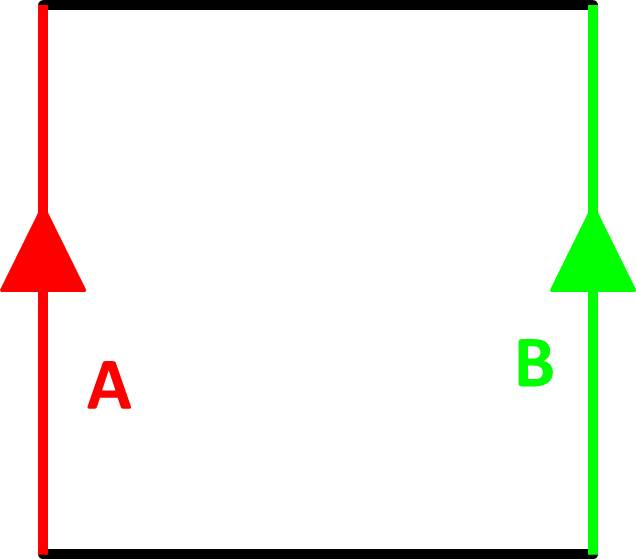
\includegraphics[scale=0.2]{images/Def_Verkleben.jpg} so heißt der Übergang zum Quotientenraum, der durch die Partition von $X$ in die Einpunktmengen von $X \backslash (A \cup B)$ und die Zweipunktmengen $\{x,f(x)\}, x \in A$ gegeben ist, \underline{Verkleben} (\underline{von $X$ längs $A$ und $B$ via des Homöomorphismus $f$}) und dieser Prozess einfach auch \underline{Verkleben von $A$ und $B$}.
\newline
\textbf{Notation:}
$$X/_{[a \sim f(a)]} \quad \text{(mit $a \in A$)}$$
\end{Kasten}


\begin{Kasten}{$n$-dimensionaler projektiver Raum}
	Der $n$-dimensionale \underline{reell-projektive} Raum\footnote{Anschaulich (projektive Geometrie): 
	Die Menge aller Geraden durch den Ursprung im $\R^{n+1}$} ist 
	$$\R \Prim^n := S^n/_{[x \sim -x]}$$
	und der $n$-dimensionale \underline{komplex-projektive} Raum ist 
	$$\C \Prim^n := \underbrace{S^{2n+1}}_{\subset \C^{n+1}}/_{[v \sim \lambda v, \lambda \in S^1]}$$
\end{Kasten}

\begin{Kasten}{homotop bezüglich der Endpunkte}
	Zwei Wege $u,v \colon I \rightarrow X$, $X$ topologischer Raum, heißen \underline{homotop} (\underline{\underline{bezüglich der Endpunkte}})
	$:\Leftrightarrow$
	\begin{enumerate}
		\item $u(0) = v(0), u(1) = v(1)$
		\item $\exists$ Homotopie $H \colon u \simeq v$ $\left(\text{mit } H(0,t) \equiv u(0), H(1,t) \equiv u(1)\right)$
	\end{enumerate}
	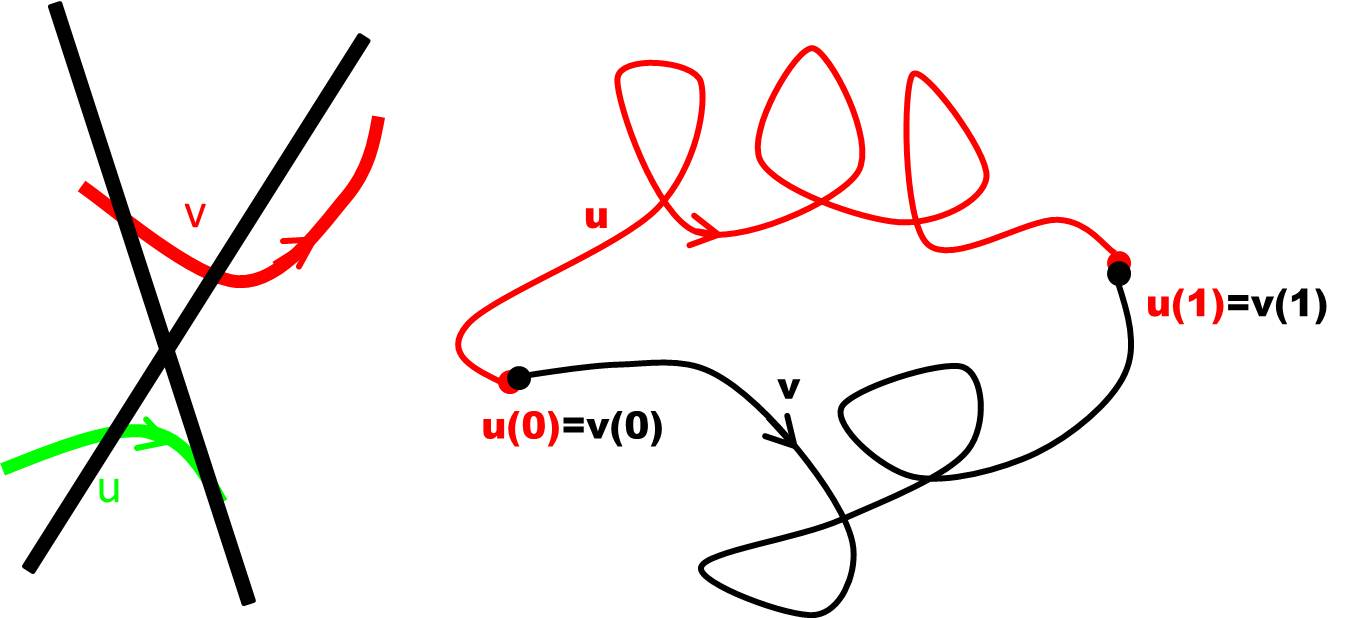
\includegraphics[scale=0.4]{images/Homotop_Endpunkte.jpg}		
\end{Kasten}

\begin{Kasten}{Produkt von Wegen}
	Sind $u$, $v$ Wege in $X$ mit $u(1)=v(0)$, so heißen $u$ und $v$ \underline{zusammensetzbar} oder \underline{aneinanderfügbar} und ihr \underline{Produkt} $u \cdot v$ ist definiert als
	$$(u \cdot v) (s) := \begin{cases} u(2s) & 0 \leq s \leq \frac{1}{2} \\ v(2s-1) & \frac{1}{2} \leq s \leq 1 \end{cases}$$
	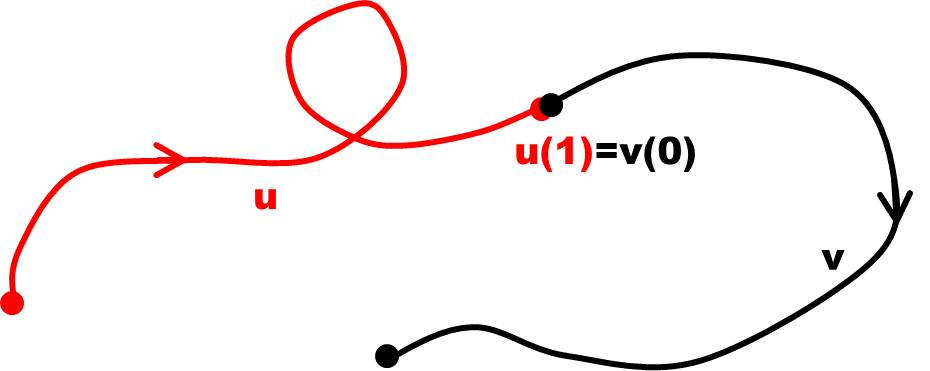
\includegraphics[scale=0.4]{images/aneinanderfuegbar.jpg}
\end{Kasten}

\begin{Kasten}{Konstanter Weg, Inverser Weg, Geschlossener Weg}
	\begin{itemize}
		\item Für $x \in X$ sei $c_x \colon I \rightarrow X$ mit $c_x \equiv x$ \underline{der konstante Weg in $x \in X$}.
		\item Für einen Weg $u \colon I \rightarrow X$ sei $u^{-1} \colon I \rightarrow X, s \mapsto u(1-s)$, der zu $u$ \underline{inverse} (oder: \underline{umgekehrt durchlaufene}) \underline{Weg}. 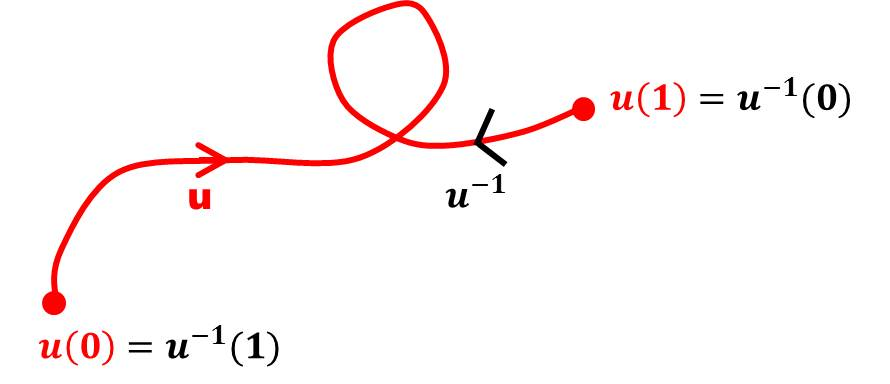
\includegraphics[scale=0.4]{images/inverser_Weg.jpg}
		\item $u \colon I \rightarrow X$ heißt \underline{geschlossener Weg} (oder: \underline{Schleife}) \underline{in $x \in X$} 
		$$:\Leftrightarrow u(0) = x = u(1)$$ 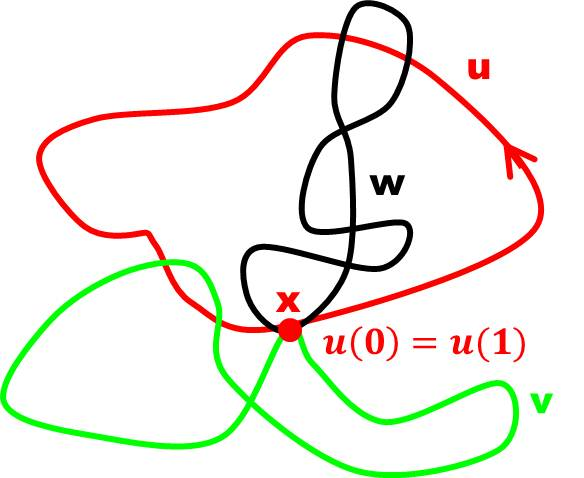
\includegraphics[scale=0.4]{images/Schleifen.jpg}
	\end{itemize}
\end{Kasten}

\begin{Kasten}{nullhomotop, einfach zusammenhängend}
	\begin{itemize}
	\item Ein geschlossener Weg $u$ in $x$ heißt \underline{nullhomotop} \newline
		$:\Leftrightarrow [u] = [c_x]$
	\item $X$ heißt \underline{einfach zusammenhängend} $:\Leftrightarrow$ \newline
	$X \text{ ist wegzusammenhängend und}$ \newline $\text{ jeder geschlossene Weg $u$ in $X$ ist nullhomotop (zu $c_{u(0)}$).}$
	\end{itemize}
\end{Kasten}

\begin{lemma}{}
	Für Wege $u,v,w \colon I \rightarrow X$ \newline mit $u(0)=x, u(1)=y=v(0), \quad v(1)=z= w(0)$ 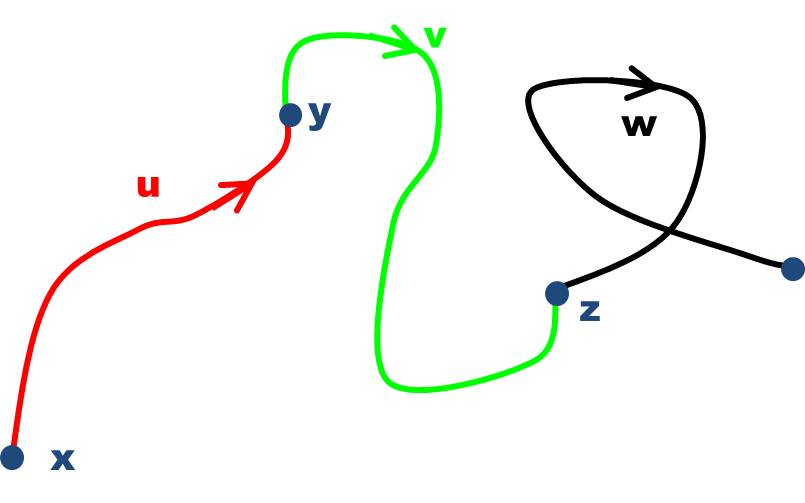
\includegraphics[scale=0.4]{images/Produkt_Lemma.jpg} gilt
	\begin{enumerate}
		\item $[u] \cdot [u^{-1}] = [u \cdot u^{-1}] = [c_x]$
		\item $[u^{-1}] \cdot [u] = [u^{-1} \cdot u] = [c_y]$
		\item $[u] \cdot [c_y] = [u] = [c_x] \cdot [u]$
		\item $[u] \cdot ([v] \cdot [w]) = ([u] \cdot [v]) \cdot [w]$
	\end{enumerate}
\end{lemma}


\begin{theorem}{}
	Für einen topologischen Raum $X$ und $x_0 \in X$ ist 
	$$\pi_1 (X,x_0) := \{ [u] \mid u \colon I \rightarrow X \text{ geschlossener Weg in } x_0 \}$$
	bezüglich $[u] \cdot [v] := [u \cdot v]$ eine Gruppe, die sogenannte \underline{Fundamentalgruppe} oder \underline{erste Homotopiegruppe} von $X$ in $x_0$. 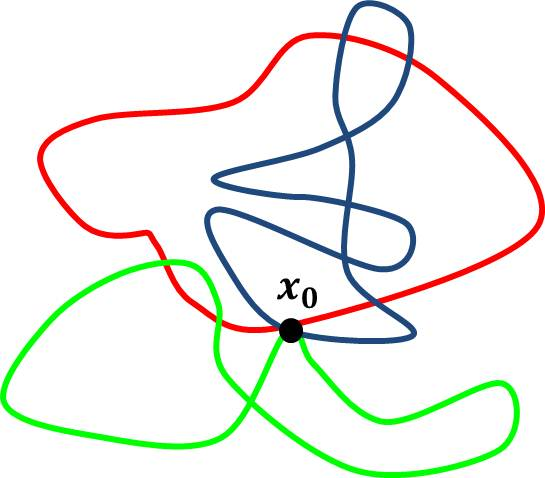
\includegraphics[scale=0.4]{images/Fundamentalgruppe.jpg}
	\newline
	Neutrales Element ist $1 = 1_{x_0} := [c_{x_0}]$ \newline und Inverses zu $\alpha = [u]$ ist $\alpha^{-1} = [u^{-1}]$.
\end{theorem}

\begin{theorem}[Unabhängigkeit vom Basispunkt]
	Ist $w \colon I \rightarrow X$ Weg von $x_0$ nach $x_1$, so ist die Abbildung 
	$$w_\# \colon \pi_1(X,x_0) \rightarrow \pi_1(X,x_1), \quad [u] \mapsto [w^{-1} \cdot u \cdot w]$$ 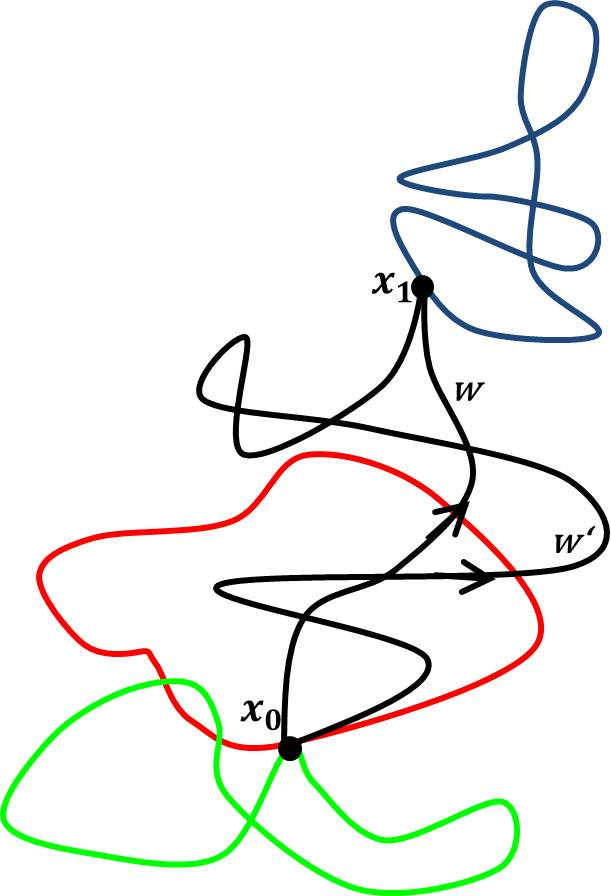
\includegraphics[scale=0.4]{images/Basispunkt_Unabhaengigkeit.jpg}
	ein \underline{Gruppen-Isomorphismus}.
\end{theorem}

\begin{Kasten}{Schleife}
	Es sei $S^1 = \{x \in \R^2 \mid ||x|| = 1\} = \{z \in \C \mid |z| = 1\}$
	und $1:= (1,0) \in S^1$ \newline 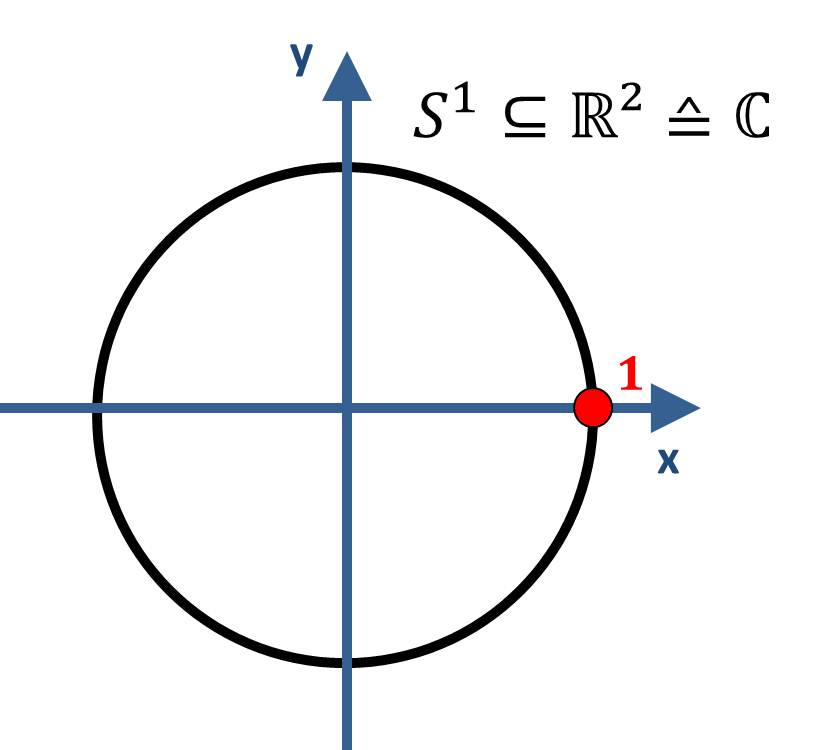
\includegraphics[scale=0.3]{images/S1_mit_1.jpg}\newline
	Eine stetige Abbildung $\gamma \colon S^1 \rightarrow X, X$ topologischer Raum, $x_0 \in X$, mit $\gamma(1)=x_0$, heißt \underline{Schleife in $x_0$}.
	 \newline 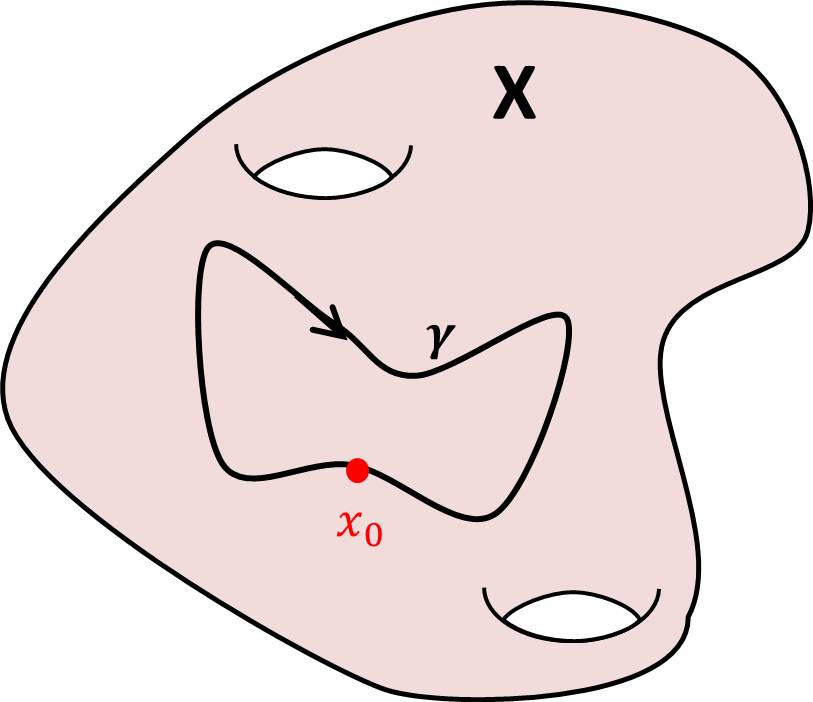
\includegraphics[scale=0.3]{images/Schleife.jpg}
\end{Kasten}

\begin{Kasten}{schleifenhomotop}
	Zwei Schleifen $\gamma, \gamma^\prime$ in $x_0$ heißen \underline{(schleifen-)homotop}, falls es eine Homotopie zwischen ihnen gibt, die auf $1 \in S^1$ stationär ist, also
	$\gamma(1) = x_0 = \gamma^\prime(1)$ die ganze Zeit festhält.
	 \newline 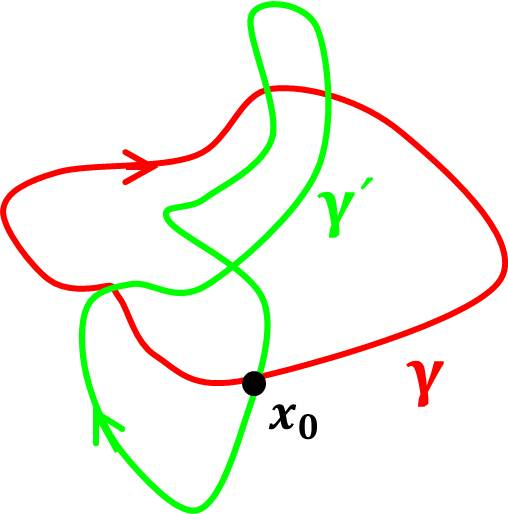
\includegraphics[scale=0.3]{images/schleifenhomotop.jpg}
\end{Kasten}

\begin{corollary}{}
	Ist $s \colon I \rightarrow X$ Weg und $\Gamma$ offene Überdeckung von $X$, so existiert eine Folge von Punkten \newline $a_1, \ldots, a_N \in I$ mit $0 = a_1 < \ldots < a_{N-1} < a_N = 1$ mit \newline $s([a_i, a_{i+1}])$ ist in einem Element von $\Gamma$ enthalten.
\end{corollary}

\begin{lemma}{}
	$\forall n \geq 2$ gilt: $\forall$ Wege $s \colon I \rightarrow S^n$ existiert eine endliche Unterteilung von $I$ in Teilintervalle, so dass die Einschränkung von $s$ auf jedes der Teilintervalle homotop zu einer Abbildung mit nirgendwo dichtem Bild ist, und zwar durch eine Homotopie, die auf den Endpunkten des Intervalls fixiert ist. (TODO: Bild 12)
	\end{lemma}
	
	
\chapter{Definitionen und Sätze aus der Übung}

\begin{Kasten}{Induzierte Topologie}
		Sei $X$ eine Menge. Sei $d \colon X \times X \rightarrow \R$ eine Metrik. Diese Metrik $d$ definiert durch folgende Bedingung eine Topologie $\OO$ auf $X$:
		\newline
		$O \subseteq X$ ist genau dann offen (d.h. $O \in \OO_d$), wenn für alle $x \in O$ ein $\epsilon > 0$ existiert mit
		$$
			B_\epsilon (x) := \{y \in X \mid d(x,y) < \epsilon\} \subseteq O.
		$$
		($B_\epsilon$ nennt man offenen $\epsilon$-Ball.)
	\end{Kasten}

\begin{Kasten}{Basis der von der Standardmetrik auf dem $\R^n$ definierten Topologie}
	$$\mathcal{B} = \{B_{\frac{1}{m}}(x) \mid x \in \Q^n, m \in \N\}$$
	Diese Basis ist abzählbar.
\end{Kasten}

	\begin{Kasten}{Homotopieäquivalenz}
		Seien $X,Y$ topologische Räume. $X$ heißt \underline{homotopieäquivalent zu Y}, falls es stetige Abbildungen $f \colon X \rightarrow Y$ und $g \colon Y \rightarrow X$ gibt, so dass $f \circ g \simeq id_Y$ und $g \circ f \simeq id_X$.
	\end{Kasten}

\begin{Kasten}{Überdeckung}
	\begin{itemize}
		\item Eine Familie $\{\mathcal{U}_\alpha \mid \alpha \in A \}$ von Teilmengen von $X$ heißt \underline{Überdeckung} von $X$, falls gilt: $X = \bigcup\limits_{\alpha \in A}{\mathcal{U}_\alpha}$.
		\item Eine Überdeckung heißt \underline{offen} (bzw. \underline{abgeschlossen}), falls alle $\mathcal{U}_\alpha (\alpha \in A)$ offen (bzw. abgeschlossen) sind.
		\item Es heißt $X$ \underline{kompakt}, falls jede offene Überdeckung $\mathcal{U}=\{U_\alpha, \alpha \in A\}$ eine endliche Teilüberdeckung $\mathcal{U}^\prime$ besitzt, d.h. es existiert $A^\prime \subset A$ endlich, so dass $\mathcal{U}^\prime = \{\mathcal{U}_\alpha \mid \alpha \in A^\prime \}$ eine offene Überdeckung von $X$ ist.
	\end{itemize}
\end{Kasten}

\begin{Kasten}{Kompakte Menge}	Eine \underline{kompakte Menge} ist eine Teilmenge eines vom Kontext her klaren topologischen Raumes, die bezüglich der Teilraumtopologie kompakt ist.
\end{Kasten}

\begin{Kasten}{Wegzusammenhang}
	\begin{itemize}
		\item Ein \underline{Weg} in $X$ ist eine stetige Abbildung $\gamma \colon I(=[0,1]) \rightarrow X$ mit Anfangspunkt $\gamma(0)$ und Endpunkt $\gamma(1)$.	
		\item Man nennt $X$ \underline{wegzusammenhängend}, falls für alle $x,y \in X$ ein Weg $\gamma \colon [0,1] \rightarrow X$ in $X$ existiert mit $\gamma(0)=x, \gamma(1)=y$.
		\item Eine \underline{Wegzusammenhangskomponente} von $X$ ist eine wegzusammenhängende Teilmenge von $X$, die in keiner echt größeren solchen Teilmenge enthalten ist.
	\end{itemize}
\end{Kasten}

\begin{Kasten}{Homotopieäquivalenz}
Für zwei topologische Räume $X,Y$ heißt eine $\underbrace{\text{stetige Abbildung }f \colon X \rightarrow Y}_{f \in C(X,Y)}$ \textbf{Homotopieäquivalenz}, falls es eine stetige Abbildung $g \colon Y \rightarrow X$ gibt, sodass $g \circ f \simeq id_x$ und $f \circ g \simeq id_Y$ gilt.
\end{Kasten}

\begin{Kasten}{homotop} Es seien $X,Y$ topologische Räume, $A \subseteq X$. Seien $f,g \in C(X,Y).$
Es heißt \underline{$f$ relativ $A$ homotop zu $g$} (in Zeichen $f \simeq g \text{ rel } A$), falls eine Homotopie $H \colon X \times I \rightarrow Y$ von $f$ nach $g$ existiert, so dass $H(a,t)=H(a,0)$ für alle $a \in A, t \in I$.
\end{Kasten}

\begin{Kasten}{kontrahierbar}
Man nennt $X$ \textbf{kontrahierbar}, falls gilt: $X \simeq \{pt\}$.
\end{Kasten}

\end{document}
